% ****** Start of file apssamp.tex ******
%
%   This file is part of the APS files in the REVTeX 4.1 distribution.
%   Version 4.1r of REVTeX, August 2010
%
%   Copyright (c) 2009, 2010 The American Physical Society.
%
%   See the REVTeX 4 README file for restrictions and more information.
%
% TeX'ing this file requires that you have AMS-LaTeX 2.0 installed
% as well as the rest of the prerequisites for REVTeX 4.1
%
% See the REVTeX 4 README file
% It also requires running BibTeX. The commands are as follows:
%
%  1)  latex apssamp.tex
%  2)  bibtex apssamp
%  3)  latex apssamp.tex
%  4)  latex apssamp.tex
%
\documentclass[%
 reprint,
%superscriptaddress,
%groupedaddress,
%unsortedaddress,
%runinaddress,
%frontmatterverbose, 
%preprint,
%showpacs,preprintnumbers,
%nofootinbib,
%nobibnotes,
%bibnotes,
 amsmath,amssymb,
 aps,
%pra,
%prb,
%rmp,
%prstab,
%prstper,
%floatfix,
]{revtex4-1}

\usepackage{graphicx}% Include figure files
\usepackage{dcolumn}% Align table columns on decimal point
\usepackage{bm}% bold math
%\usepackage{hyperref}% add hypertext capabilities
%\usepackage[mathlines]{lineno}% Enable numbering of text and display math
%\linenumbers\relax % Commence numbering lines

%\usepackage[showframe,%Uncomment any one of the following lines to test 
%%scale=0.7, marginratio={1:1, 2:3}, ignoreall,% default settings
%%text={7in,10in},centering,
%%margin=1.5in,
%%total={6.5in,8.75in}, top=1.2in, left=0.9in, includefoot,
%%height=10in,a5paper,hmargin={3cm,0.8in},
%]{geometry}
\usepackage{pstricks,pst-node}
\usepackage[utf8]{inputenc}
\usepackage{float}
\usepackage[spanish]{babel}
\usepackage{amsmath}
\usepackage{hyperref}
\usepackage{tikz}
\usetikzlibrary{shapes.geometric, arrows}
\tikzstyle{startstop} = [rectangle, rounded corners, minimum width=3cm, minimum height=1cm,text centered, text width=2.5cm, draw=black, fill=magenta!10]
\tikzstyle{io} = [trapezium, trapezium left angle=70, trapezium right angle=110, minimum width=3cm, minimum height=1cm, text centered, text width=2.3cm, draw=black, fill=blue!10]
\tikzstyle{process} = [rectangle, minimum width=3cm, minimum height=1cm, text centered, text width=3cm, draw=black, fill=cyan!10]
\tikzstyle{decision} = [diamond, minimum width=3cm, minimum height=1cm, text centered, draw=black, text width=2.3cm,  fill=lime!20]
\tikzstyle{arrow} = [thick,->,>=stealth]

\begin{document}

\title{Efecto fotoeléctrico}% Force line breaks with \\
\thanks{Estudio sobre el efecto fotoeléctrico estudiado por Einstein y probado experimental por Millikan. Dado este experimento, se plantea la relación entre la emisión de electrones y la energía de los fotones.}%

\author{Maria Sofía Álvarez López}%
\homepage{ms.alvarezl@uniandes.edu.co}
\affiliation{
 Universidad de los Andes\\
}%

\author{Sara María Varón Echeverri}
\homepage{sm.varon@uniandes.edu.co}
\affiliation{
Universidad de los Andes\\
}%

\date{\today}% It is always \today, today,
             %  but any date may be explicitly specified

\begin{abstract}
El objetivo de éste laboratorio fue estudiar la emisión de electrones a través de una superficie metálica iluminada. Dicho objetivo fue completado al medir valores de corriente versus voltaje en cuatro bombillos LED de diversos colores. Al entender la corriente como un flujo de electrones, se podría entonces estudiar su emisión conforme a la frecuencia de la luz transmitida. Posteriormente, se utilizaron dichos electrones para determinar la energía de los fotones incidentes para cada uno de los cuatro colores, teniendo en cuenta el valor absoluto de la carga de un electrón. Adicionalmente, al comparar dichos valores energéticos, se demostró cómo la energía de los fotones dependen del color, mostrando cómo los colores más fríos como el azul cargan más energía que los cálidos como el rojo. Ésto se debe a la frecuencia con la cuál las ondas de cada color se disipan, no de la intensidad. Esto fue demostrado al comparar datos de un mismo bombillo a dos intensidades distintas. Tras el análisis cualitativo correspondiente, se aproximó el valor de la constante de Planck (h) a un valor de $5.13278 \times 10^{-34} \pm 1.23076 \times 10^{39}$ eV*s y el valor de la función del trabajo del metal $Cs_3Sb$ a $1.9126 \times 10^{-19}$ $\phi$eV, relativamente cercanos a los valores reales.
\end{abstract}

\pacs{Valid PACS appear here}% PACS, the Physics and Astronomy
                             % Classification Scheme.
%\keywords{Suggested keywords}%Use showkeys class option if keyword
                              %display desired
\maketitle

%\tableofcontents

\section{\label{intro} Introducción y estado del arte}

En 1905, tras los avances de la mecánica cuántica y el desarrollo de diversas pruebas correspondientes a la Teoría de la relatividad especial, "Einstein supuso que la radiación incidente consistía en paquetes de energía localizada $E = h \gamma$ que viajaba a la velocidad de la luz" \cite{Einstein}. Dado lo anterior, el resultado de la interacción entre un haz de luz y una superficie metálica puede tener dos resultados:

\begin{enumerate}
    \item Los fotones responden a la óptica.
    \item Los fotones desaparecen ya que ceden toda su energía con el fin de sacar los electrones.
\end{enumerate}

Años después, en 1914, Millikan hizo la primera prueba experimental para demostrar la existencia de los fotones y estimar una aproximación para la constante de Planck. En concreto, la pendiente de sus gráficas se acercaron con un error ínfimo al valor teórico de la constante de Planck, $h = 6,625 \times 10^{-34} Js$ \cite{Millikan}.

De la teoría de Einstein y la experimentación de Millikan se puede deducir que la energía de los electrones liberados es igual a las ecuación \eqref{(2)}, teniendo en cuenta que la carga del electrón $-1.60217656535 \times 10^{-19}$ C. De la ecuación anterior se deduce que parte de la energía se transporta a la superficie y que hay una energía asociada con $\phi$ que es la energía mínima que necesita un electrón para pasar por el metal, como se muestra en la \ref{fig:trabajo_metal}. 

\begin{equation}\label{(2)}
  K_{max} = h \gamma - \phi = \frac{1}{2} m v^2
\end{equation}

\begin{figure}[H]
    \centering
    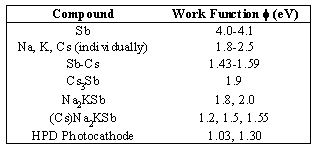
\includegraphics[scale= 0.5]{Trabajo_del_metal.png}
    \caption{Tabla del trabajo con el que el electrón está ligado a un metal definido. Ésta gráfica es el resultado del estudio desarrollado por Craig Savage \cite{funcion_de_trabajo_del_metal}. Para el desarrollo de nuestro experimento se utilizó un bombillo IP39 hecho de $Cs_3Sb$.}
    \label{fig:trabajo_metal}
\end{figure}

Como resumen del efecto fotoeléctrico se pueden considerar los siguientes postulados como relevantes para el experimento a realizar \cite{Einstein}:

\begin{enumerate}
    \item El número de electrones liberados es proporcional a la intensidad de las radiaciones incidentes.
    \item La energía cinética máxima de los fotoelectrones depende de la frecuencia y no de la intensidad de luz.
    \item $K_max$ tiene una relación lineal con $\gamma$ dada la ecuación \eqref{(2)}.
    \item La potencia de frenado $V_0$ depende de la función de trabajo.
    \item Existe una frecuencia umbral $\gamma_0$ por debajo de la cual no ocurre el efecto fotoeléctrico.
    \item La emisión ocurre instantáneamente cuando la frecuencia supera la frecuencia umbral $\gamma_0$.
 \end{enumerate}

Para el siguiente montaje se utilizarán: una celda fotoeléctrica, LEDs de varios colores, una fuente de voltaje y un micro-amperímetro. Los LEDs ha utilizar son rojo (659 nm), ambar (590 nm), verde (567 nm) y azul (469 nm). La razón por la cuál se utilizan este tipo de bombillos y no otros es por su luminosidad y que pueden encenderse en menos de 1 $\mu s$ que responde de forma beneficiosa al tiempo de respuesta de los experimentos \cite{LEDs}.

Cabe mencionar las diversas fuentes de error de ésta manera de estudiar el efecto fotoeléctrico \cite{Errores_asociados_new_approach}. Por un lado, es necesario que la superficie metálica sea completamente pura y que sus alrededores estén vacíos, en otras palabras, que la superficie sea pura y se encuentre al vació. Adicionalmente, se deben eliminar las corrientes oscuras que afectan los datos de las corrientes reales y el deterioro espacio-carga que se genera entre dos electrodos. Respecto a la luz utilizada, es necesario confirmar la pureza espectral y que la intensidad lumínica sea constante. Demostrado así, existen fuentes de error en varios momentos del experimento y, por esto, pueden existir discrepancias con la teoría establecida con anterioridad.

\section{\label{montaje} Montaje experimental}

Para este experimento se utilizó el diagrama circuital mostrado en la Figura \ref{fig:Figura 2}.
\begin{figure}[H]
    \centering
    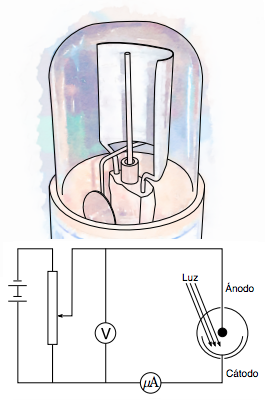
\includegraphics[scale= 0.4]{Montaje.png}
    \caption{Diagrama del circuito armado. Cabe notar que no incluye el alimentador de los LEDs ni del amperímetro.}
    \label{fig:Figura 2}
\end{figure}
Para la realización de este experimento, primero fue necesario conectar todo el circuito mostrado previamente (en la figura \ref{fig:Figura 2}) con mucho cuidado, para asegurar un desarrollo exitoso del experimento. \\ 
Antes de poner los LEDs en la fotocelda, se verificó que ella funcionara, notando que el micro-amperímetro acusara una corriente que debía reducir al cubrir la fotocelda.\\
Primero, fue necesario ajustar el cero de la escala del microamperímetro, de la siguiente manera: 
\begin{enumerate}
    \item Para que no hubiera corriente, se desconectó el cable que unía al microamperímetro con la fotocelda. 
    \item Se mantuvo oprimido el botón rojo (para maximizar la sensibilidad del experimento).
    \item Se giró la perilla \textit{"zero adjust"} hasta que la aguja indicara cero. En este paso, nuestro microamperímetro no alcanzó a llegar hasta cero, lo cual puede representar una fuente de error sistemático en nuestra toma de datos.
\end{enumerate}

Más adelante, sobre la celda fotoeléctrica se colocó una caperuza que, además de contener varios LEDs de colores (rojo, ámbar, verde y azul), también excluía la luz del ambiente. Se conectaron los LEDs al circuito y se buscó asegurar que la caperuza no se moviera durante la medición, para evitar errores aleatororios que causaran que la luz no tuviese intensidad constante. Lo anterior pues, al mover la caperuza, se afectaba el área de incidencia de la luz, cambiando, también, la intensidad medida.\\
Por otro lado, el voltaje de frenado se ovtuvo de una fuente fijada en 2 voltios. Esta se varió usando el potenciómetro instalado junto a la celda. Esta cantidad fue medida con el voltímetro, mostrando en la figura \ref{fig:Figura 2}. \\
De vuelta al microamperímetro, se empezó a observar la corriente de los electrones emitidos. El voltaje de frenado era aumentado para lograr corrientes desde 10 hasta 0.5 ($\times 10^{-8} A$), en intervalos de $0.5 A$. Para cada corriente, se anotaron los voltajes correspondientes. Con el fin de lograr medir corrientes más pequeñas, se oprimió el botón rojo que aumentaba 10 veces la sensibilidad del micro-amperímetro. Se siguió aumentando el voltaje de frenado para medir corrientes y sus respectivos voltajes. Con estos datos, y construyendo regresiones lineales y predicciones adecuadas, se logró determinar el voltaje de corte que justamente anula la corriente. \\
Finalmente, para uno de los colores,se repitió la medición con una intensidad diferente. Lo anterior, se logró girando los LEDs para que no iluminaran a la celda de frente. Con esto, se observió que la corriente disminuye, pero el voltaje de corte sigue siendo el mismo, lo cual implica que no depende de la intensidad de la luz, como se explicará más adelante.



\section{\label{resultados} Resultados y análisis}

Con el fin de estudiar la emisión de electrones a través de una superficie metálica iluminada, se utilizó un tubo de efecto fotoeléctrico para calcular la corriente y el voltaje de diversas lámparas LED, más específicamente, de colores rojo, ambar, verde y azul. Según la Ley de Ohm, la relación entre voltaje y corriente corresponde a $V=IR$ y por tanto, al graficar el voltaje contra la corriente se podría encontrar la resistencia de cada uno de los bombillos en la forma de $\frac{1}{R}$. Por esta razón, los datos obtenidos debían tener un comportamiento lineal necesariamente. Adicionalmente, con el fin de de obtener el voltaje de corte (en el que la corriente es cero), se extrapolan las gráficas. Dado uno de los postulados del efecto fotoeléctrico, debe tenerse en cuenta que existe una frecuencia umbral $\gamma_0$ por debajo de la cual no ocurre el efecto fotoeléctrico y por tanto, es necesario extrapolar cada gráfica para obtener los valores asociados a ese momento. 

\begin{figure}[H]
    \centering
    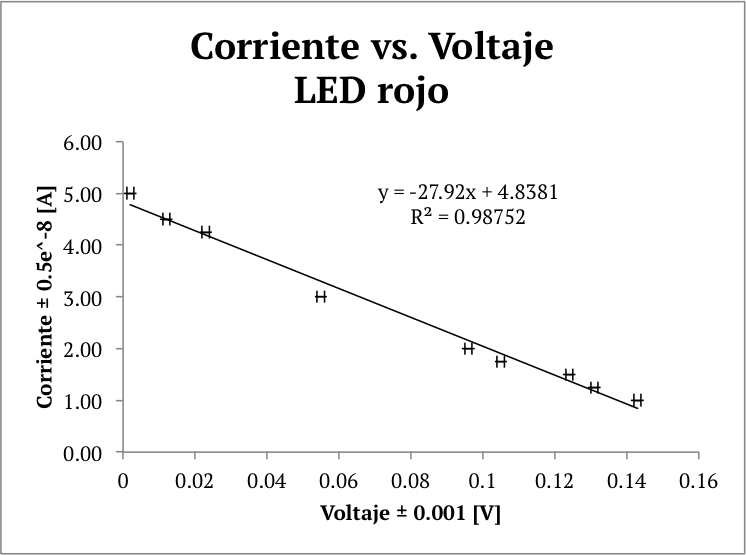
\includegraphics[scale= 0.6]{ROJO.png}
    \caption{Diagrama obtenido al graficar los datos de corriente vs. voltaje para el LED de color rojo. Debe tenerse en cuenta que los datos mostrados no son todos los datos obtenidos. Varios datos fueron eliminados porque tenían un gran porcentaje de error aleatorio. Dado que las incertidumbres asociadas con los instrumentos eran insignificantes, las gráficas sólo muestran pequeñas barras de incertidumbre al rededor de sus puntos.}
    \label{fig:rojo}
\end{figure}

\begin{figure}[H]
    \centering
    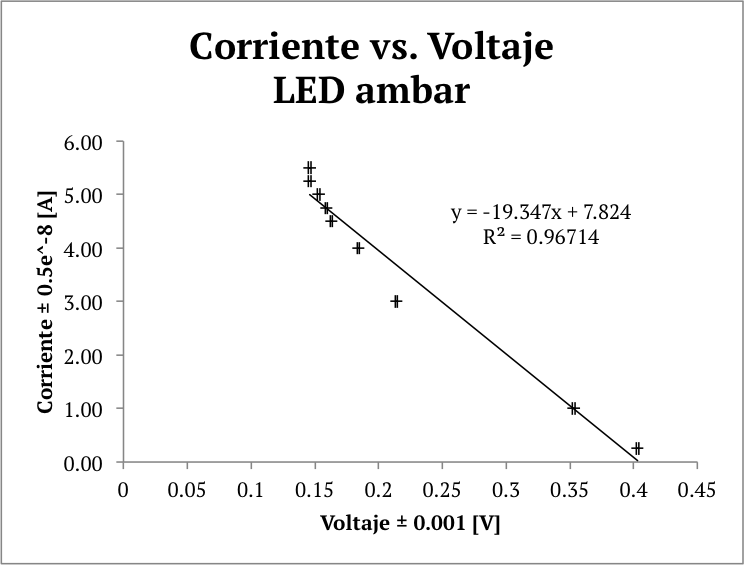
\includegraphics[scale= 0.6]{AMBAR.png}
    \caption{Diagrama obtenido al graficar los datos de corriente vs. voltaje para el LED de color ambar. Debe tenerse en cuenta que los datos mostrados no son todos los datos obtenidos. Varios datos fueron eliminados porque tenían un gran porcentaje de error aleatorio. Dado que las incertidumbres asociadas con los instrumentos eran insignificantes, las gráficas sólo muestran pequeñas barras de incertidumbre al rededor de sus puntos.}
    \label{fig:ambar}
\end{figure}

\begin{figure}[H]
    \centering
    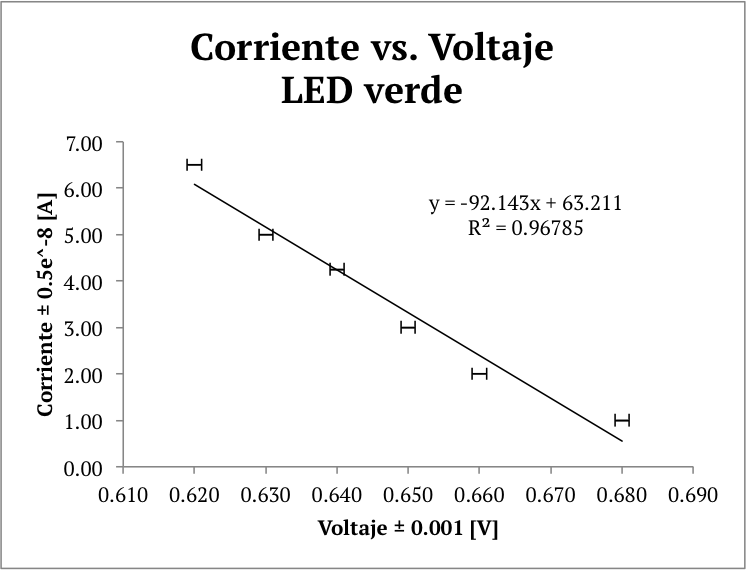
\includegraphics[scale= 0.6]{VERDE.png}
    \caption{Diagrama obtenido al graficar los datos de corriente vs. voltaje para el LED de color verde. Debe tenerse en cuenta que los datos mostrados no fueron modificados ni seleccionados dada la poca cantidad de datos obtenidos para el bombillo de éste color. Dado que las incertidumbres asociadas con los instrumentos eran insignificantes, las gráficas sólo muestran pequeñas barras de incertidumbre al rededor de sus puntos.}
    \label{fig:verde}
\end{figure}

Para el LED azul se utilizaron dos intensidades distintas para la toma de datos con el fin de mostrar la relevancia de la intensidad en el efecto fotoeléctrico. Mencionado anteriormente como uno de los principales postulados del efecto fotoeléctrico, la energía cinética máxima de los foto-electrones depende de la frecuencia y no de la intensidad de luz. Para el análisis de estos datos se debe tener en cuenta que hubo diversos datos extremos que salen de manera abrupta de la línea de tendencia. El principal motivo por el cual se dieron estos datos fue la sensibilidad de los instrumentos de medida. Al efectuar la medición los datos cambiaban bruscamente en el voltímetro y el amperímetro. Como si existiera la posibilidad de un daño en el aparato, la variación de los datos declara la impresión de los datos. Adicionalmente, debe tenerse en cuenta que la medida de incertidumbre varía con respecto al nivel de sensibilidad del aparato. No sólo la exactitud sino la precisión fueron comprometidas en este experimento.

\begin{figure}[H]
    \centering
    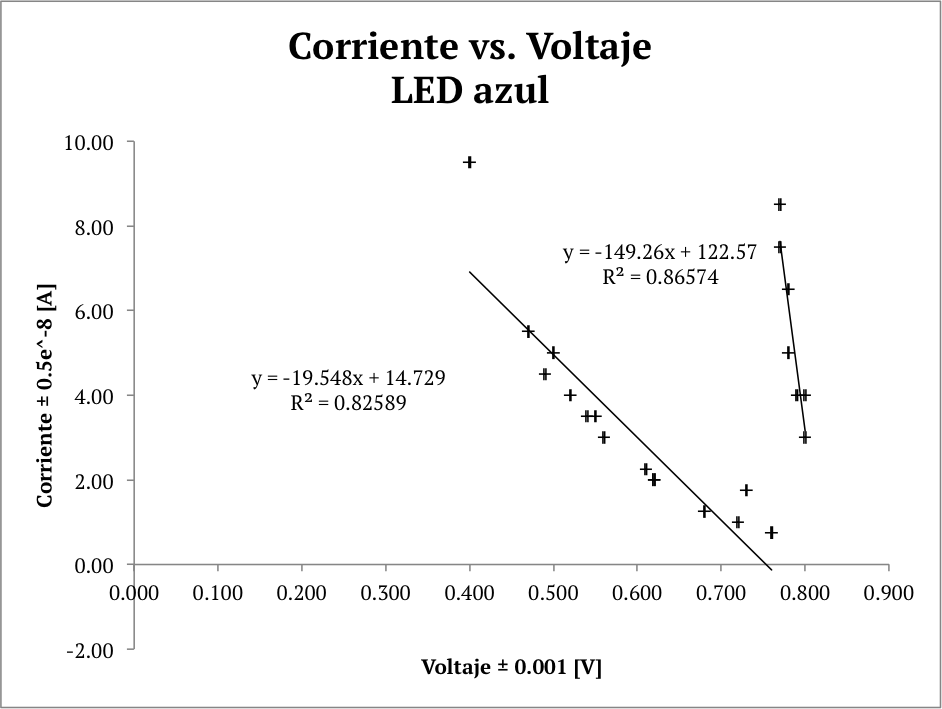
\includegraphics[scale= 0.53]{AZUL.png}
    \caption{Diagrama obtenido al graficar los datos de corriente vs. voltaje para el LED de color azul con dos intensidades distintas. Debe tenerse en cuenta que los datos mostrados no fueron modificados ni seleccionados. Dado que las incertidumbres asociadas con los instrumentos eran insignificantes, las gráficas sólo muestran pequeñas barras de incertidumbre al rededor de sus puntos.}
    \label{fig:azules}
\end{figure}

Visto ya en la gráfica \ref{fig:azules}, los valores presentados parecerían muy distintos a plena vista. Sin embargo, al notar los datos en el cuadro \ref{tab:intesidades azul}, se puede ver con claridad que la desviación estándar de la energía de los fotones para cara una de las intensidades es muy pequeña, casi no varían los datos. Esto significa entonces que tienen voltajes de corte muy cercanos entre sí y cuyas diferencias pueden venir principalmente de las fuentes de error previamente mencionadas. Esto significa entonces que un mismo color con una misma frecuencia, sin importar la intensidad de luz que esté emanando, responden al mismo voltaje de corte y por tanto a la misma energía.

\begin{table}[H]
  \centering
  \caption{En la siguiente tabla se muestran los resultados tras el análisis para las dos intensidades del bombillo LED azul. La desviación estándar de los datos obtenidos aparece ser insignificante, por tanto, se encuentra que la intensidad no afecta realmente los datos. La posible razón por la cual existe discrepancia reside en la incertidumbre de los elementos de medición, además de los errores experimentales que acarrean el experimento.}
    \begin{tabular}{|r|r|r|r|}
    \hline
    {Intensidad} & {Voltaje de} & {Energía fotones} & {Desviación} \\
          & {corte [V]} & {[eV]} & {estándar} \\
    \hline
    1     & 0.788 & 1.263E-19 & 3.742E-21 \\
    2     & 0.821 & 1.316E-19 &  \\
    \hline
    \end{tabular}
  \label{tab:intesidades azul}
\end{table}

\begin{figure}[H]
    \centering
    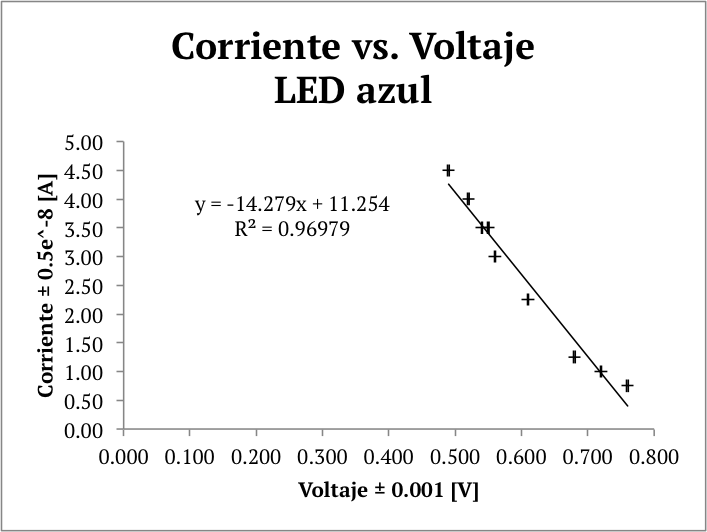
\includegraphics[scale= 0.6]{Azul_mejorado.png}
    \caption{Diagrama obtenido al graficar los datos de corriente vs. voltaje para el LED de color azul para una de las intensidades. Se eligió ésta intensidad dado que se tenían muchos más datos y podría entonces generarse un mejor análisis con respecto a los resultados de la línea de tendencia. Debe tenerse en cuenta que los datos mostrados no son todos los datos obtenidos, Varios datos fueron eliminados porque tenían un gran porcentaje de error aleatorio. Dado que las incertidumbres asociadas con los instrumentos eran insignificantes, las gráficas sólo muestran pequeñas barras de incertidumbre al rededor de sus puntos.}
    \label{fig:azul}
\end{figure}

Asimismo, resulta conveniente analizar las gráficas de los residuales, para cada conjunto de datos de corriente vs voltaje, con el fin de determinar si el ajuste lineal fue el más adecuado. De esta manera, 

\begin{figure}[H]
    \centering
    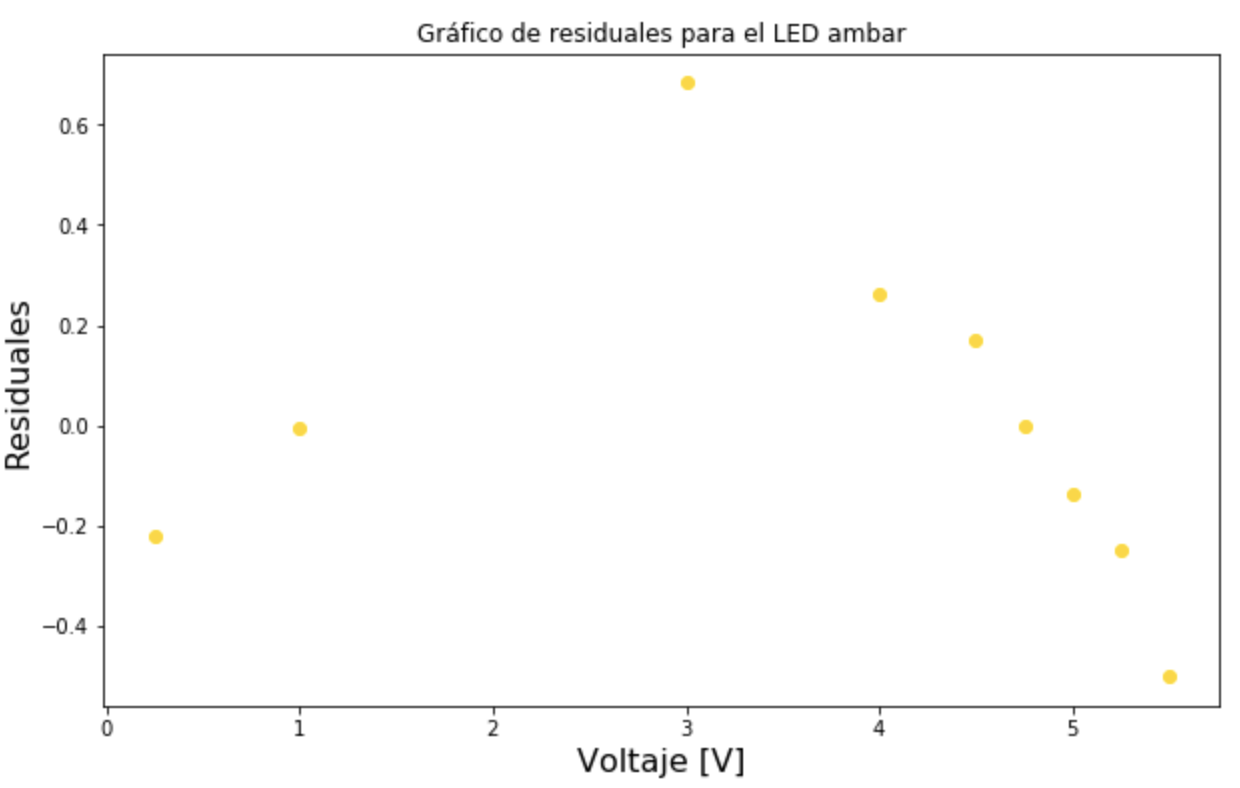
\includegraphics[scale= 0.34]{resLEDambar.png}
    \caption{Diagrama obtenido al graficar los residuales de corriente y voltaje para la luz ambar. Como puede notarse, los datos tienen una distribución aleatoria, lo cual sustenta el ajuste lineal utilizado.}
    \label{fig:ambarRes}
\end{figure}

\begin{figure}[H]
    \centering
    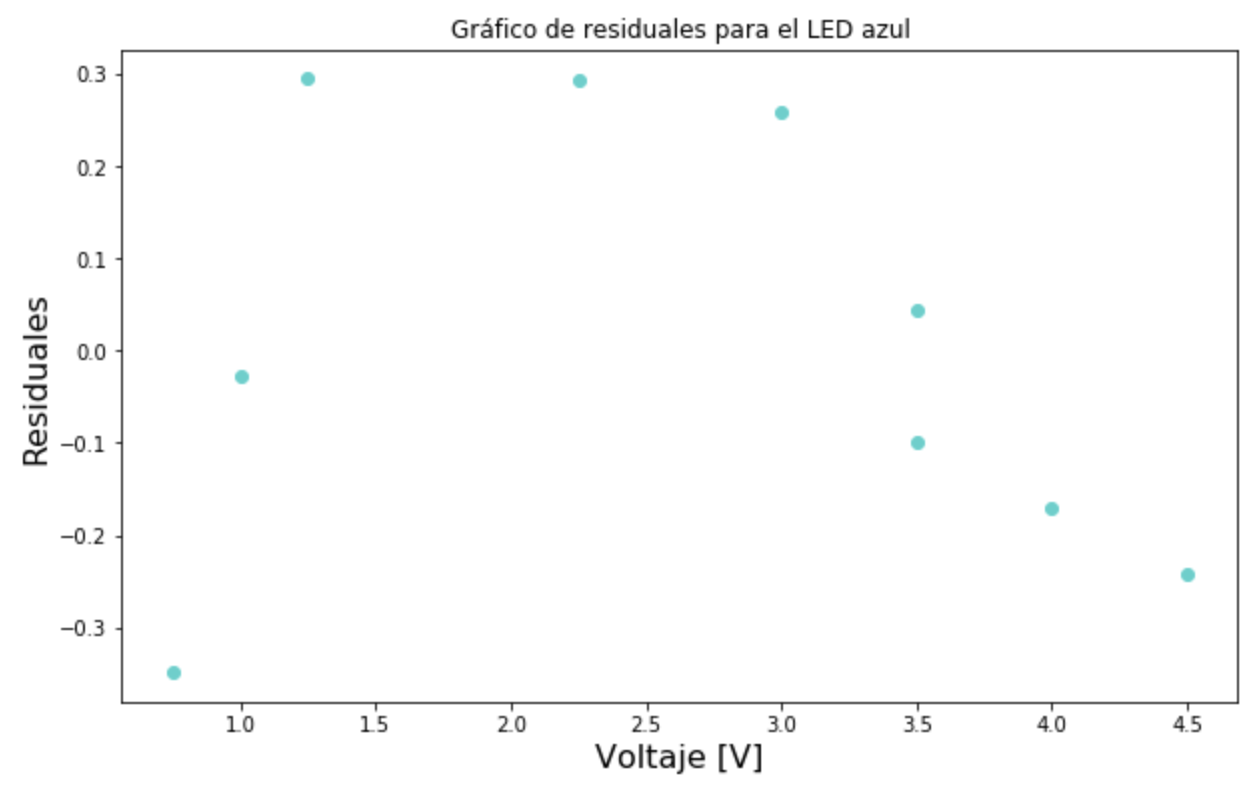
\includegraphics[scale= 0.34]{resLEDazul.png}
    \caption{Diagrama obtenido al graficar los residuales de corriente y voltaje para la luz azul. Como puede notarse, los datos tienen una distribución aleatoria, lo cual sustenta el ajuste lineal utilizado.}
    \label{fig:ambarRes}
\end{figure}

\begin{figure}[H]
    \centering
    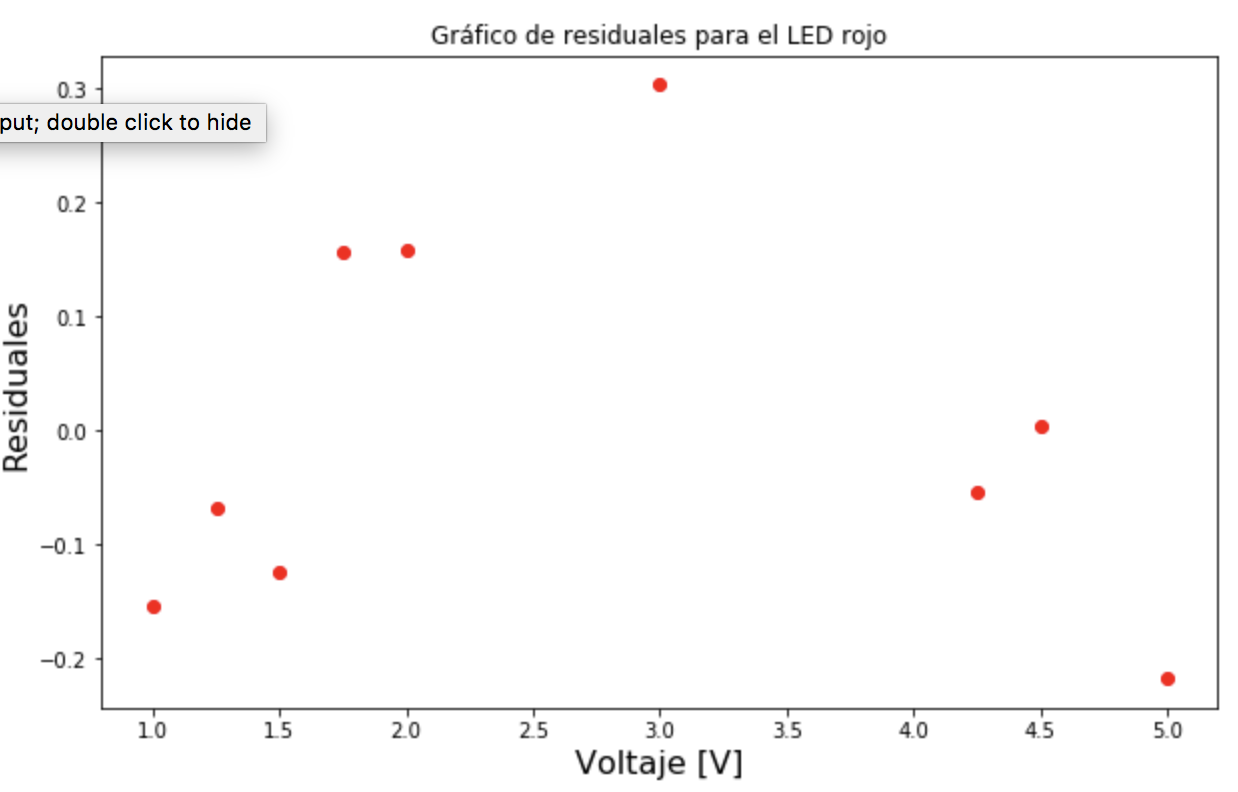
\includegraphics[scale= 0.34]{resLEDrojo.png}
    \caption{Diagrama obtenido al graficar los residuales de corriente y voltaje para la luz roja. Como puede notarse, los datos tienen una distribución aleatoria, lo cual sustenta el ajuste lineal utilizado.}
    \label{fig:ambarRes}
\end{figure}

\begin{figure}[H]
    \centering
    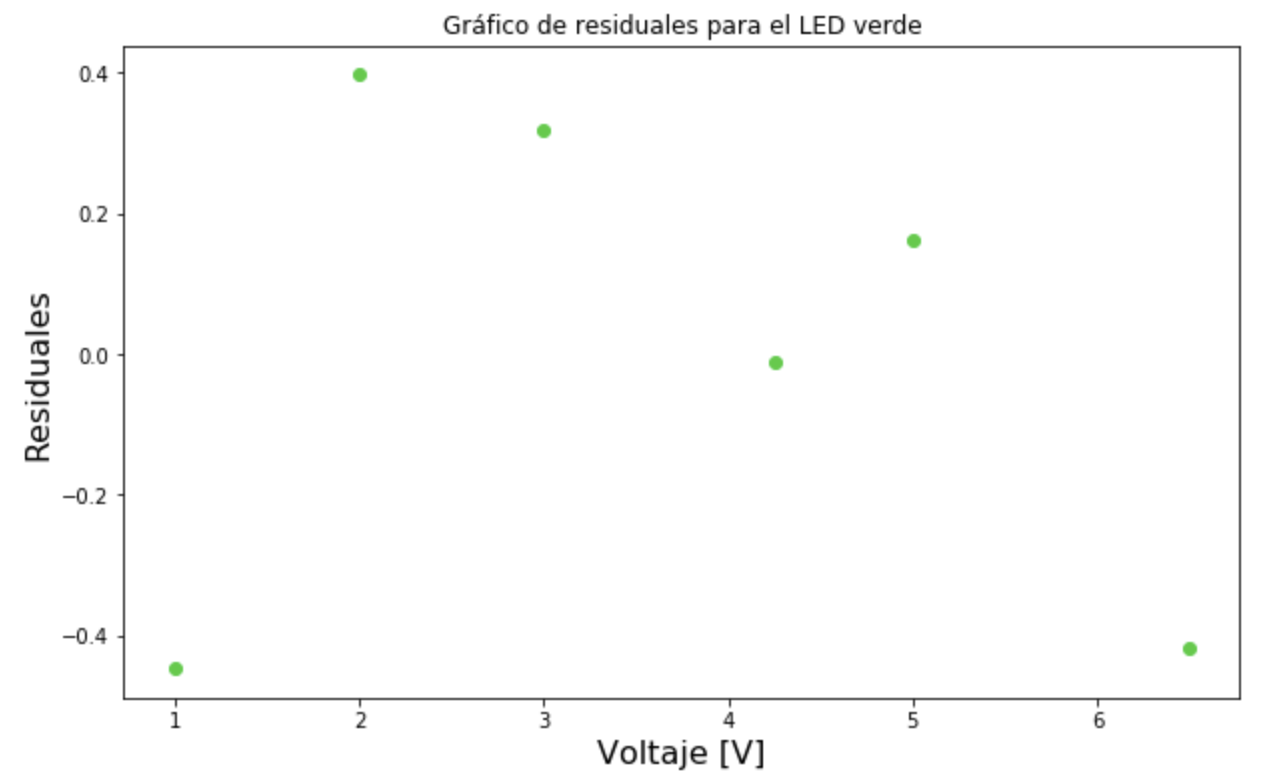
\includegraphics[scale= 0.34]{resLEDverde.png}
    \caption{Diagrama obtenido al graficar los residuales de corriente y voltaje para la luz verde. Como puede notarse, los datos tienen una distribución aleatoria, lo cual sustenta el ajuste lineal utilizado.}
    \label{fig:ambarRes}
\end{figure}

De esta manera, puede notarse que, como los datos de los residuales tuvieron una distribuc
ón aleatoria, el ajuste lineal era el más adecuado para este caso. \\

Dados los datos de las longitudes de ondasi emitidas por los LEDs medidos por Benjamín Oostra y conforme a la relación $Frecuencia = \frac{c}{\lambda}$, se calcula la frecuencia para cada uno de los colores de LED dados. Adicionalmente, de las gráficas realizadas se puede encontrar una relación entre los electrones y la energía de los fotones incidentes. Al medir el voltaje de corte y multiplicarlo por la carga absoluta de un electrón se obtiene la energía máxima de los electrones. La razón de éste fenómeno es que el voltaje implica una diferencia de potencial entre placas, y el producto entre la diferencia de potencial y la carga es igual al trabajo que aplica un electrón en frenar. Para el voltaje de corte ningún electrón pasa de una placa a la otra, y por esto, la energía potencia de los electrones, en ese momento, es igual a la cinética. Al graficar estos datos, como en la figura \ref{fig:constante de Planck}, se ve que los datos responden a un ajuste lineal cuya pendiente debe ser igual a la constante de Planck, cuyo corte con el eje x responde a la frecuencia mínima (anteriormente llamada $\gamma_0$) que marca el umbral del efecto fotoeléctrico, y la “función de trabajo” del material en el tubo. 

\begin{table}[H]
  \centering
  \caption{Procesamiento de datos para la estimación de la constante de Planck. Las constantes utilizadas para dicho proceso fueron: la constante de la velocidad de la luz (c), que es igual a $299,792,458 ms^-1$, y el valor absoluto de la carga de un electrón, que es igual a $1.60217656535E-19 C$.}
    \begin{tabular}{|r|r|r|r|}
    \hline
    \multicolumn{1}{|c|}{Longitud de onda} & \multicolumn{1}{c|}{Voltaje de corte} & \multicolumn{1}{c|}{Energía} & \multicolumn{1}{c|}{Frecuencia} \\
    \multicolumn{1}{|c|}{$\pm$ 3 E-7 m} & \multicolumn{1}{c|}{$\pm 0.001 V$} & \multicolumn{1}{c|}{fotones} & \multicolumn{1}{c|}{ ($\frac{c}{\lambda}$)} \\
    \hline
    0.000000659 & 0.173 & 2.776E-20 & 4.5492E+14 \\
    0.000000590 & 0.404 & 6.479E-20 & 5.08123E+14 \\
    0.000000567 & 0.686 & 1.099E-19 & 5.28734E+14 \\
    0.000000469 & 0.788 & 1.263E-19 & 6.39216E+14 \\
    0.000000469 & 0.821 & 1.316E-19 & 6.39216E+14 \\
    \hline
    \end{tabular}
  \label{tab:constante de Planck}
\end{table}

\begin{figure}[H]
    \centering
    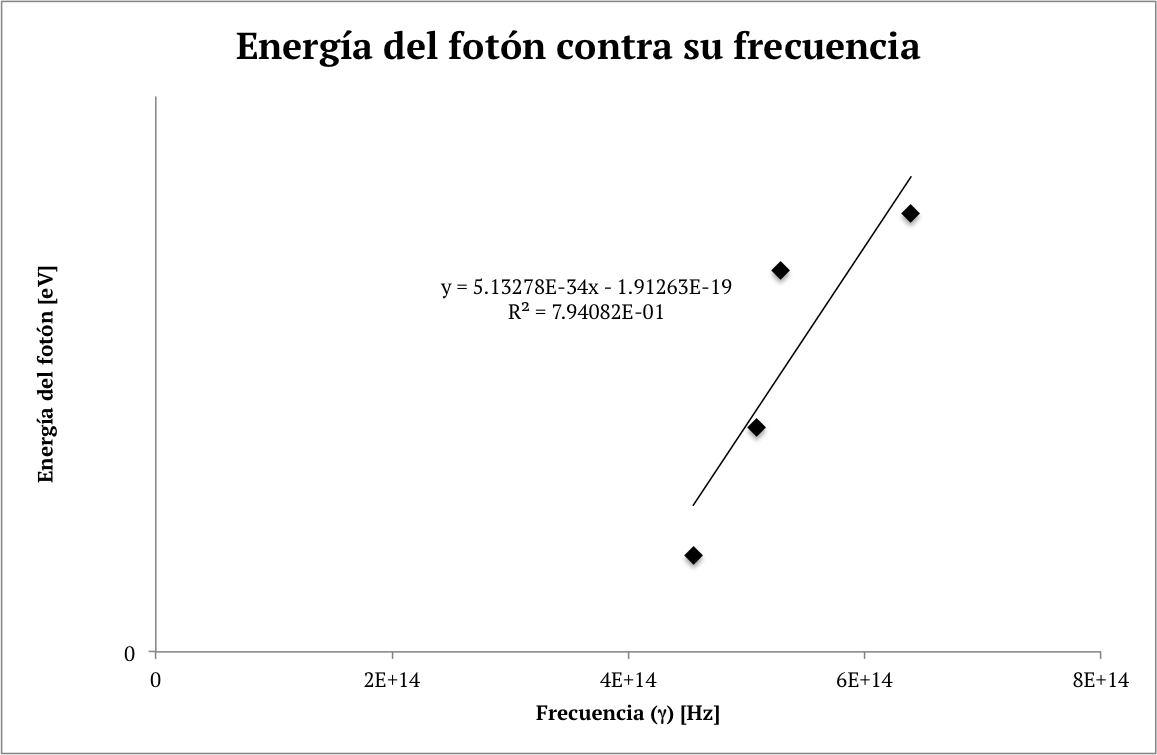
\includegraphics[scale=0.40]{energiavsfrecuencia.png}
    \caption{Diagrama obtenido al graficar los datos calculados de la energía de los fotones [eV] y la frecuencia de los mismos [Hz]. Teniendo en cuenta uno de los postulados del efecto fotoeléctrico, la energía cinética máxima de los electrones es igual a la energía de los fotones y tiene una relación lineal con la frecuencia ($\gamma$) dada la ecuación \eqref{(2)} y su pendiente es la constante de Planck.}
    \label{fig:constante de Planck}
\end{figure}

Como consecuencia de la explicación anterior y los datos mostrados en la gráfica \ref{fig:constante de Planck}, la constante de Planck para nuestro experimento tendría una aproximación de $5.13278 \times 10^{-34}$, con respecto al valor real igual a $6.62607015 \times 10^{-34}$. Si se hiciera un análisis de error de este valor sería igual a $22.54 \%$, aparentemente alto dada la prueba sencilla que se hizo. Sin embargo, cabe aclarar que las incertidumbres y los errores experimentales mencionados con anterioridad pudieron afectar gravemente el resultado, llevándolo a este tipo de desfaces del valor natural. Adicional a esto, el punto de corte presenta un valor de $1.9126 \times 10^{-19}$, haciendo alusión al valor de la función de trabajo del metal en cuestión, en este caso, $Cs_3Sb$. Al comparar este resultado con el de otros estudios, por ejemplo, el de Craig Savage \cite{funcion_de_trabajo_del_metal}, se encuentra una discrepancia de únicamente el $0.66 \%$. Dado el desarrollo del experimento y los errores asociados a los demás resultados, se puede decir que el resultado obtenido para este valor es excepcional y su error es despreciable en comparación con el error en otros datos obtenidos.

\section{\label{conclusiones} Conclusiones}

En conclusión, se estudió con satisfacción la emisión de electrones a través de una superficie metálica iluminada, en este caso, de la lámpara de LED IP39 hecha de $Cs_3Sb$. La relación entre la corriente y el voltaje de diversos colores de LED expuestos a ésta lámpara probó ser un método satisfactorio para estudiar la emisión de electrones conforme a la frecuencia de la luz transmitida. Por radiación, el metal en cuestión libera electrones al ser expuesto a un rayo de luz cuando el voltaje sobrepasa el voltaje mínimo para que existan los fotoeléctrones. El desprendimiento de electrones, pues, se entiende como una corriente eléctrica. 

Adicionalmente, como fue explicado en la introducción, el producto entre el valor absoluto de la carga del electrón y el voltaje de corte sería igual a la energía de los fotones incidentes. Dado que cada haz de luz difiere en color y por tanto genera un desprendimiento de electrones distinto en el material, se utilizaron dichos electrones para determinar y comparar las energías de los fotones incidentes, como bien se muestran en las gráficas \ref{fig:rojo}, \ref{fig:ambar}, \ref{fig:verde} y \ref{fig:azul}. Este proceso implicó tener diversas fuentes de error que afectaron los resultados del experimento. Por un lado, la incertidumbre de las medidas y por otro, la variación rápida de las mediciones causan errores sistemáticos y no sistemáticos en la toma de datos.

Como resultado de la comparación entre los distintos valores energéticos obtenidos y expuestos en la tabla \ref{tab:constante de Planck}, se demostró cómo la energía de los fotones dependen del color, mostrando cómo los colores más fríos como el azul cargan más energía que los cálidos como el rojo. Ésto se debe a que el color es una expresión física de la frecuencia con la cuál las ondas de cada color se disipan. Cada color tiene una cantidad de energía asociada distintamente. 

Cabe aclarar entonces, la frecuencia afecta la energía pero la intensidad de luz no. Esto fue demostrado al comparar datos de un mismo bombillo a dos intensidades distintas, mostrado en la gráfica \ref{fig:azules}. Si se toma la desviación estándar de los cálculos de energía mostrados en la tabla \ref{tab:intesidades azul}, se encuentra entonces que existe una ínfima diferencia entre las energías transferidas, estimada en un valor de $3.742 \times 10^{-21}$ eV. Éste desface pudo darse por diversas fuentes de error o, también, por la poca cantidad de datos para la segunda intensidad. La energía, entonces, sólo depende de la frecuencia del haz de luz y no de su intensidad.

Tras el análisis cuantitativo de la relación entre la energía y la frecuencia de los colores utilizados en la gráfica \ref{fig:constante de Planck}, se aproximó el valor de la constante de Planck (h) a un valor de $5.13278 \times 10^{-34} \times 10^{39}$ eV*s, teniendo en cuenta la ecuación descrita por Einstein como $E=hf$. Teniendo en cuenta que el valor teórico de dicha constante es igual a $6.62607015 \times 10^{-34}$ eV*s, el error asociado a esta medida fue de $22.5\%$. Por otro lado, el valor de la función del trabajo del metal $Cs_3Sb$ a $1.9126 \times 10^{-19}$ $\phi$eV, y el valor esperado era de $1.9 \times 10^{-19}$ $\phi$eV. Teniendo en cuenta lo anterior, el error asociado a la medida de la función del trabajo fue igual a $0.66\%$. Como consecuencia, los valores obtenidos son efectivamente concordantes con la teoría y responden de manera eficaz a la teoría descrita por Einstein. Aunque existieron errores en la toma de datos y en el desarrollo del experimento, el resultado se muestra satisfactorio.

\bibliography{biblio}

\end{document}